\documentclass[letterpaper,11pt]{article}
\usepackage{graphicx}
\usepackage{listings}
\usepackage[super]{nth}
\usepackage[hyphens]{url}
\usepackage{amsmath}
\usepackage[makeroom]{cancel}
\usepackage[table]{xcolor}
\usepackage{comment}
\usepackage[space]{grffile}

\lstset{
	basicstyle=\footnotesize,
	breaklines=true,
}

\begin{document}

\begin{titlepage}

\begin{center}

\Huge{Assignment 4}

\Large{CS 595:  Introduction to Web Science}

\Large{Fall 2013}

\Large{Shawn M. Jones}

\Large Finished on \today

\end{center}

\end{titlepage}

\newpage
\section*{1}

\subsection*{Question}

\begin{verbatim}
1.  From your list of 1000 links, choose 100 and extract all of the
links from those 100 pages to other pages.  We're looking for user 
navigable links, that is in the form of: 

<A href="foo">bar</a>

We're not looking for embedded images, scripts, <link> elements,
etc.  You'll probably want to use BeautifulSoup for this.

For each URI, create a text file of all of the outbound links from
that page to other URIs (use any syntax that is easy for you).  For
example:

site: 
http://www.cs.odu.edu/~mln/    
links:
http://www.cs.odu.edu/
http://www.odu.edu/
http://www.cs.odu.edu/~mln/research/
http://www.cs.odu.edu/~mln/pubs/
http://ws-dl.blogspot.com/
http://ws-dl.blogspot.com/2013/09/2013-09-09-ms-thesis-http-mailbox.html
etc.

Upload these 100 files to github (they don't have to be in your report).
\end{verbatim}

\newpage
\subsection*{Answer}

To get the 100 links, I decided it was likely that \verb+cnn.com+ would likely link to itself a lot, so I typed the following command to extract 100 of those entries from my \verb+shalist-final.txt+ file from Assignment 3.
\begin{lstlisting}[frame=single,basicstyle=\tiny]
grep "cnn.com" shalist-final.txt | head -n 100 > pages-to-extract.txt
\end{lstlisting}

The program for extracting the links from the given list of pages is in Listing \ref{lst:q1code}.  It is executed as follows
\begin{lstlisting}[frame=single,basicstyle=\tiny]
./getLinks.py pages-to-extract.txt ../../assignment3/q1/collection linkFiles
\end{lstlisting}

The first argument is a file containing the list of URIs and SHA hashes.  The second argument is the directory to search through for the files with the name corresponding to the SHA hashes contained in the file from the first argument.  The last argument is the directory to write the link information out to.

Once this is done, the \verb+linkFiles+ directory contains files like \newline \verb+f25db00c9aeb80bb92f465cd7794536d87889958.links.json+ which are single key JSON dictionaries containing the URI and the URIs the representation links to.

I chose JSON because it should be relatively easy to parse for Question 2, and also because the test for question 1 states ``use any syntax that is easy for you''.  I wanted to save time and not write my own parser when Python has one built in.  On the first pass, I had the script generate one large JSON file, which could easily be read for Question 2, and would work well for our 100 links.  But having the script write out a file per URI scales better when we look at millions of URIs, especially if there is a bug in the script or hardware failure.

The function on line 62 extracts the links using BeautifulSoup, and the first pass at this script stopped there.  Once I examined the output, I realized that there were a large number of relative URIs, JavaScript links, URIs missing complete paths, etc.  This caused the creation of the function on line 12, which tries to account for that madness.



\newpage
\lstinputlisting[language=Python,frame=single,caption={Python program for printing out links from 100 pages},label=lst:q1code,captionpos=b,numbers=left,showspaces=false,showstringspaces=false,basicstyle=\footnotesize]{q1/getLinks.py}

\newpage
\section*{2}

\subsection*{Question}

\begin{verbatim}
2.  Using these 100 files, create a single GraphViz "dot" file of
the resulting graph.  Learn about dot at:

Examples:
http://www.graphviz.org/content/unix
http://www.graphviz.org/Gallery/directed/unix.gv.txt

Manual:
http://www.graphviz.org/Documentation/dotguide.pdf

Reference:
http://www.graphviz.org/content/dot-language
http://www.graphviz.org/Documentation.php

Note: you'll have to put explicit labels on the graph, see:
https://gephi.org/users/supported-graph-formats/graphviz-dot-format/

(note: actually, I'll allow any of the formats listed here:

https://gephi.org/users/supported-graph-formats/

but "dot" is probably the simplest.)
\end{verbatim}

\newpage
\subsection*{Answer}

Because I stored the data from Question 1 in JSON format, the script for Question 2 is much smaller.  It was run like so:

\begin{lstlisting}[frame=single]
./makeDot.py ../q1/linkFiles > linkGraph.dot
\end{lstlisting}
where the first argument is the directory to search for the JSON files from Question 1.  The script prints to \verb+stdout+ so a redirect creates the DOT file.

The script is shown in Listing \ref{lst:q2code}.  Lines 27-29 print the DOT code for each edge, with labels.  Line 10 prints the opening DOT block and line 31 prints the close to the block.

\lstinputlisting[language=Python,frame=single,caption={Python program for printing converting links from Question 1 into a DOT file},label=lst:q2code,captionpos=b,numbers=left,showspaces=false,showstringspaces=false,basicstyle=\footnotesize]{q2/makeDot.py}


\newpage
\section*{3}

\subsection*{Question}

\begin{verbatim}
3.  Download and install Gephi:

https://gephi.org/

Load the dot file created in #2 and use Gephi to:

- visualize the graph (you'll have to turn on labels)
- calculate HITS and PageRank
- avg degree
- network diameter
- connected components

Put the resulting graphs in your report.

You might need to choose the 100 sites with an eye toward
creating a graph with at least one component that is nicely
connected.  You can probably do this by selecting some portion
of your links (e.g., 25, 50) from the same site.  
\end{verbatim}

\newpage
\subsection*{Answer}

The graph described by the dot file in Question 2 contains $4276$ nodes and $11488$ edges.

From Gephi, visualizing the graph produced a horrid monstrosity shown in Figure \ref{fig:q3vis-hairball}.  Choosing all of my links from CNN is what led to this.  The shaving on the right and left are not actually unconnected edges.  Gephi appears to have cropped the image on export.

After using the \emph{Yifan Hu} layout, the graph became the much better, as shown in Figure \ref{fig:q3vis-yifan-hu}.  It turns out that each of the subgraphs in the CNN graph somewhat correspond to parts of the CNN site (and outbound links).  Some of these have been colorized to demonstrate this phenomenon.  Green corresponds to URIs with \verb+eatocracy.cnn.com+, red-orange is \verb+ac360.blogs.cnn.com+, purple is \verb+crossfire.blogs.cnn.com+.  The blue-yellow and violet-yellow groups on the lower left part of the graph correspond to \verb+fortune.cnn.com+ and \verb+money.cnn.com+ respectively.  Unfortunately, Gephi did not have enough colors to convey all of the subgroups.

All of CNN's pages link to the same template menu links, which explains much of the strongly connected parts.  I expected most of the pages to link to pages in the center of the graph, but I did not expect this much ``clumping''.

Because of this clumping Figure \ref{fig:q3hits-authorities} shows low authority scores on all pages, and Figure \ref{fig:q3hits-hubs} shows what look to be four hubs, but are likely so many data points crammed into these four scores.  Also, the PageRank for all pages approaches $0$, as shown in Figure \ref{fig:q3pagerank} because so many of the pages link to one another.

\begin{figure}[p]
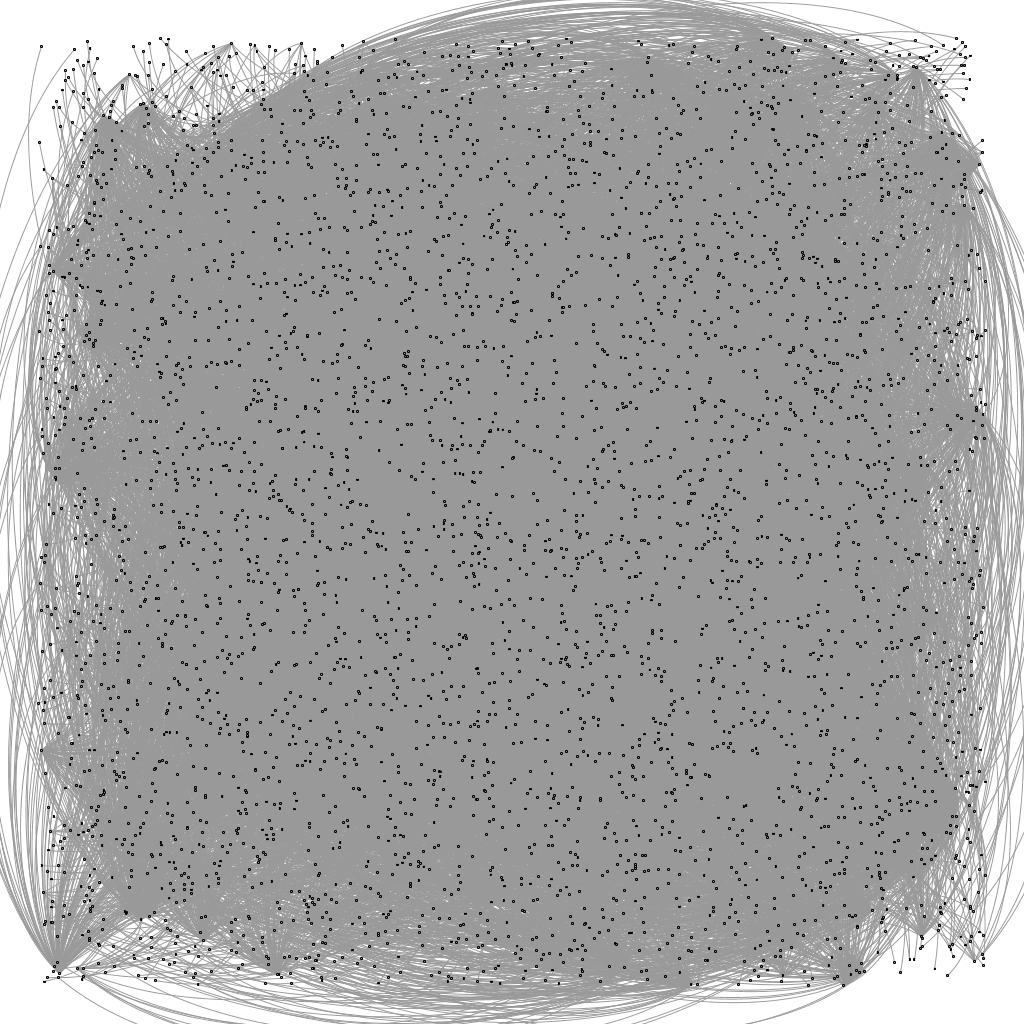
\includegraphics[scale=0.3]{q3/Visualized/visualized.png}
\caption{Initial Visualization of the Dot file produced from Question 2}
\label{fig:q3vis-hairball}
\end{figure}

\begin{figure}[p]
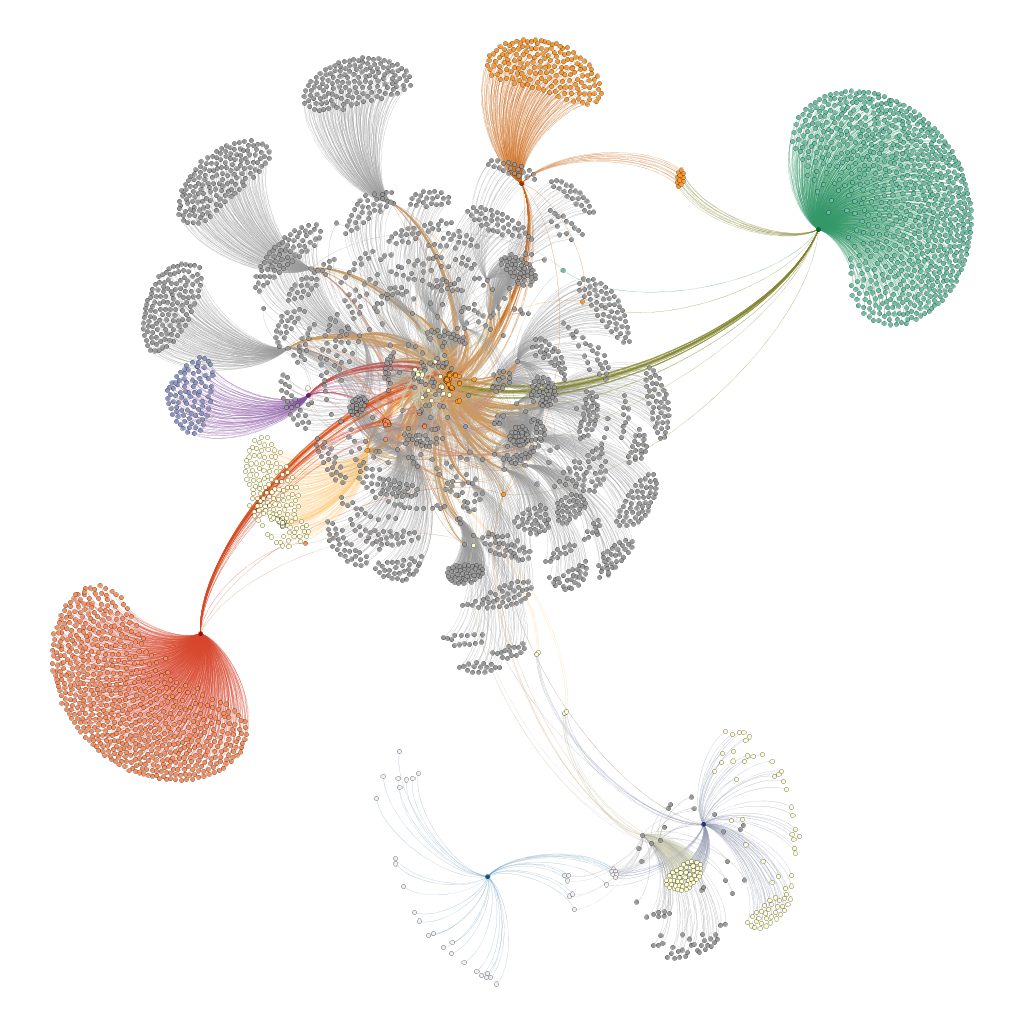
\includegraphics[scale=0.4]{q3/Visualized/colorized-yifan-hu-visualized.png}
\caption{Yifan Hu Visualization of the Dot file produced from Question 2}
\label{fig:q3vis-yifan-hu}
\end{figure}

\begin{figure}[p]
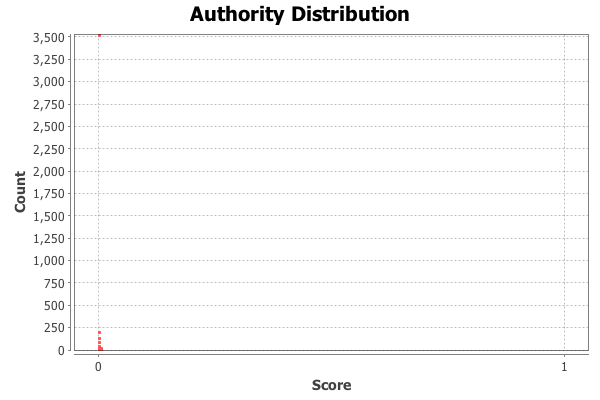
\includegraphics[scale=0.5]{q3/HITS/authorities.png}
\caption{Plot of the HITS authorities from the Dot file produced from Question 2}
\label{fig:q3hits-authorities}
\end{figure}

\begin{figure}[p]
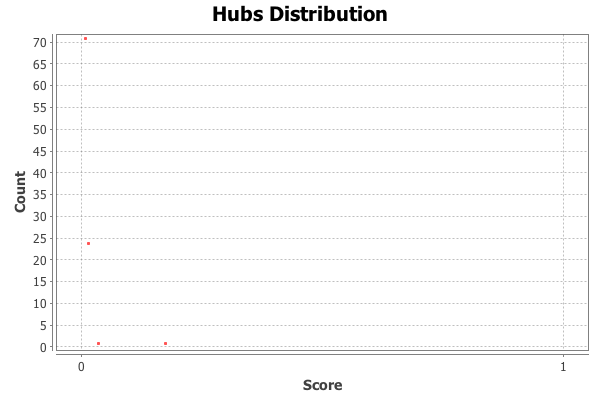
\includegraphics[scale=0.5]{q3/HITS/hubs.png}
\caption{Plot of the HITS hubs from the Dot file produced from Question 2}
\label{fig:q3hits-hubs}
\end{figure}

\begin{figure}[p]
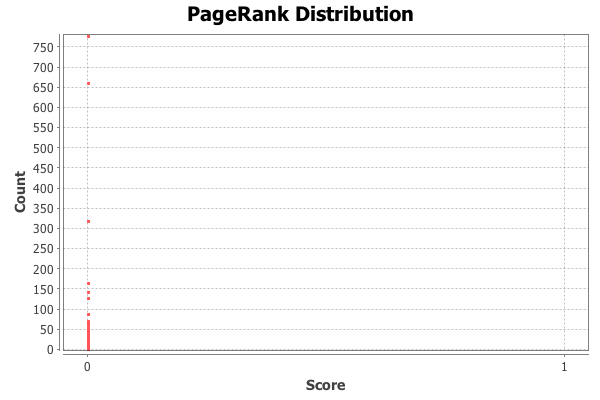
\includegraphics[scale=0.5]{q3/PageRank/pageranks.png}
\caption{Plot of PageRank from the Dot file produced from Question 2}
\label{fig:q3pagerank}
\end{figure}

\begin{figure}[p]
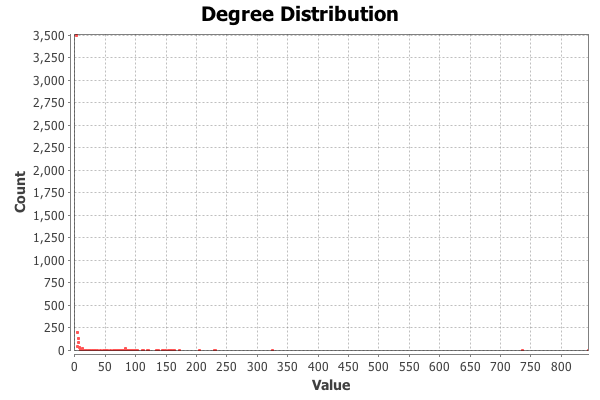
\includegraphics[scale=0.5]{q3/Avg-Degree/degree-distribution.png}
\caption{Plot of the Avg Degree Distribution from the Dot file produced from Question 2}
\label{fig:q3avgdegree-distribution}
\end{figure}

\begin{figure}[p]
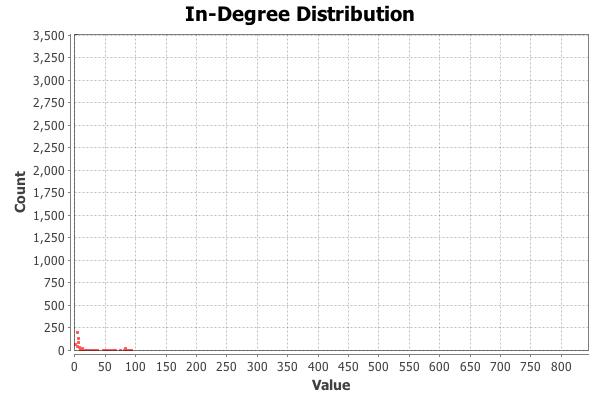
\includegraphics[scale=0.5]{q3/Avg-Degree/indegree-distribution.png}
\caption{Plot of the Avg Degree Indegree Distribution from the Dot file produced from Question 2}
\label{fig:q3avgdegree-indegree-distribution}
\end{figure}

\begin{figure}[p]
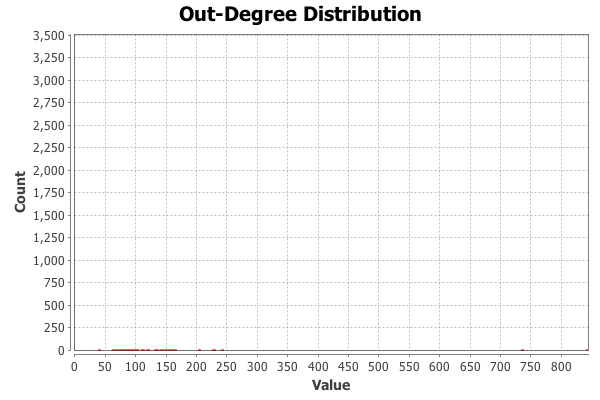
\includegraphics[scale=0.5]{q3/Avg-Degree/outdegree-distribution.png}
\caption{Plot of the Avg Degree Outdegree Distribution from the Dot file produced from Question 2}
\label{fig:q3avgdegree-outdegree-distribution}
\end{figure}

\begin{figure}[p]
\includegraphics[scale=0.5]{"q3/Network-Diameter/Betweenness Centrality Distribution"}
\caption{Plot of the Network Diameter Betweenness Centrality Distribution from the Dot file produced from Question 2}
\label{fig:q3netdiam-betweenness}
\end{figure}

\begin{figure}[p]
\includegraphics[scale=0.5]{"q3/Network-Diameter/Closeness Centrality Distribution"}
\caption{Plot of the Network Diameter Closeness Centrality Distribution from the Dot file produced from Question 2}
\label{fig:q3netdiam-closeness}
\end{figure}

\begin{figure}[p]
\includegraphics[scale=0.5]{"q3/Network-Diameter/Eccentricity Distribution"}
\caption{Plot of the Network Diameter Eccentricity Distribution from the Dot file produced from Question 2}
\label{fig:q3netdiam-eccentricity}
\end{figure}

\begin{figure}[p]
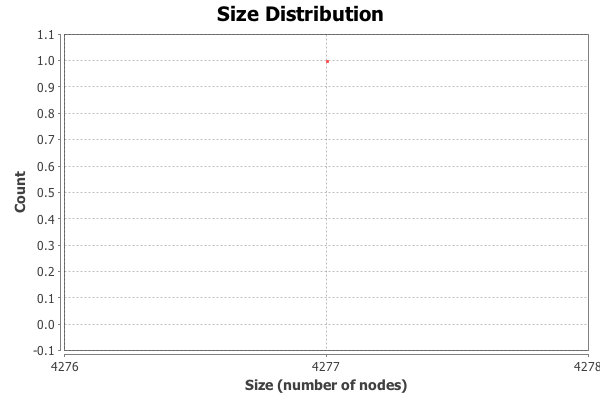
\includegraphics[scale=0.5]{q3/Connected-Components/cc-size-distribution.png}
\caption{Plot of the Connected Components from the Dot file produced from Question 2}
\label{fig:q3cc}
\end{figure}

\clearpage
\bibliographystyle{acm}
\bibliography{references}

\end{document}